% Midterm report of the Mesocosm project.
% The numbers of the steganographic-collusion study are read from the generated files of that study's report
% (../steganographic-collusion/generated). The other numbers are copied from the project's evidence documents
% and from the repository on the report's date; the report states that date.
% Build: pdflatex report.tex twice, from this directory.
\documentclass[11pt,a4paper]{article}
\usepackage[T1]{fontenc}
\usepackage[utf8]{inputenc}
\usepackage{lmodern}
\usepackage[margin=1in]{geometry}
\usepackage{microtype}
\usepackage{booktabs}
\usepackage{tabularx}
\usepackage{array}
\usepackage{enumitem}
\usepackage{float}
\usepackage{placeins}
\usepackage[font=small,labelfont=bf,skip=6pt]{caption}
\captionsetup[table]{position=top}
\usepackage{xcolor}
\usepackage{tikz}
\usetikzlibrary{arrows.meta,positioning,fit}
\usepackage{pgfplots}
\pgfplotsset{compat=1.18}
\usepackage[colorlinks=true,linkcolor=black,citecolor=black,urlcolor=black]{hyperref}

\newcommand{\ShortCycles}{100}
\newcommand{\ShortUpdates}{700}
\newcommand{\ShortSenderUpdates}{500}
\newcommand{\ShortReceiverUpdates}{200}
\newcommand{\ShortTexts}{1,920}
\newcommand{\ShortTaskSuccess}{0.575}
\newcommand{\ShortBypass}{0.927}
\newcommand{\ShortFlaggedPercent}{7.3}
\newcommand{\ShortAccBad}{0.419}
\newcommand{\ShortAccGood}{0.735}
\newcommand{\ShortRewardTotal}{0.204}
\newcommand{\ShortRewardTask}{$-$0.060}
\newcommand{\ShortRewardOverseer}{0.164}
\newcommand{\ShortRewardLength}{0.100}
\newcommand{\ShortMinutes}{295}
\newcommand{\ShortHours}{4.9}
\newcommand{\ShortPeakMemory}{29.8}
\newcommand{\LongCycles}{200}
\newcommand{\LongUpdates}{1,400}
\newcommand{\LongSenderUpdates}{1,000}
\newcommand{\LongReceiverUpdates}{400}
\newcommand{\LongTexts}{1,920}
\newcommand{\LongTaskSuccess}{0.998}
\newcommand{\LongBypass}{0.994}
\newcommand{\LongFlaggedPercent}{0.6}
\newcommand{\LongAccBad}{0.996}
\newcommand{\LongAccGood}{1.000}
\newcommand{\LongRewardTotal}{1.276}
\newcommand{\LongRewardTask}{0.984}
\newcommand{\LongRewardOverseer}{0.193}
\newcommand{\LongRewardLength}{0.100}
\newcommand{\LongMinutes}{580}
\newcommand{\LongHours}{9.7}
\newcommand{\LongPeakMemory}{29.8}
\newcommand{\Seed}{3385207819}
\newcommand{\SecondsPerCycle}{173}
\newcommand{\SameNumbers}{28,580}
\newcommand{\SameTexts}{5,376}
\newcommand{\SenderBatch}{128}
\newcommand{\SenderGroup}{16}
\newcommand{\ReceiverBatch}{128}
\newcommand{\KlCoef}{0.1}
\newcommand{\TargetKl}{30}
\newcommand{\OutputMin}{15}
\newcommand{\OutputMax}{20}
\newcommand{\OverseerScale}{0.2}
\newcommand{\LengthScale}{0.1}
\newcommand{\ReceiverUpdatesPerCycle}{2}
\newcommand{\SenderUpdatesPerCycle}{5}
\newcommand{\OverseerCheckAccuracy}{0.973}
\newcommand{\OverseerCheckTexts}{148}
\newcommand{\OverseerThreshold}{0.75}
\newcommand{\EarlyCycles}{110}
\newcommand{\EarlyBlockMin}{0.498}
\newcommand{\EarlyBlockMax}{0.568}
\newcommand{\FlaggedPeak}{0.476}
\newcommand{\FlaggedPeakCycles}{11 to 20}
\newcommand{\FlaggedAtHundred}{0.081}
\newcommand{\FlaggedLast}{0.008}
\newcommand{\AccuracyLast}{0.995}
\newcommand{\RiseSixty}{124}
\newcommand{\RiseNinety}{142}
\newcommand{\RiseNinetyFive}{146}
\newcommand{\HeldRiseUpdate}{800}
\newcommand{\HeldRiseAccuracy}{0.656}
\newcommand{\HeldConvergedUpdate}{1,050}
\newcommand{\HeldConvergedAccuracy}{0.969}
\newcommand{\HeldTexts}{128}
\newcommand{\HeldEvaluations}{28}
\newcommand{\PublishedRiseEnd}{860}
\newcommand{\DelayUpdates}{190}
\newcommand{\DelayCycles}{27}
\newcommand{\EndTexts}{512}
\newcommand{\EndBad}{259}
\newcommand{\EndBadFirst}{1}
\newcommand{\EndBadQuote}{199}
\newcommand{\EndGood}{253}
\newcommand{\EndGoodFirst}{253}
\newcommand{\EndGoodQuote}{4}
\newcommand{\EndUniversityWords}{0}
\newcommand{\EndNegative}{4}
\newcommand{\MiddleTexts}{512}
\newcommand{\MiddleUniversityWords}{27}
\newcommand{\MiddleNegative}{44}
\newcommand{\MiddleBoth}{22}
\newcommand{\OpenGoodStart}{0.157}
\newcommand{\OpenBadStart}{0.088}
\newcommand{\OpenGoodThousand}{148 of 179}
\newcommand{\OpenBadThousand}{9 of 205}
\newcommand{\QuoteBadEarly}{52 of 188}
\newcommand{\QuoteBadDip}{4 of 184}
\newcommand{\AllGoodFromUpdate}{1,200}
\newcommand{\QuoteMajorityUpdate}{1,300}
\newcommand{\HeldAtQuoteMajority}{0.992}


\definecolor{seriesA}{HTML}{2A78D6}
\definecolor{seriesB}{HTML}{EB6834}
\definecolor{inksecondary}{HTML}{52514E}
\definecolor{gridgray}{HTML}{E4E3DF}
\definecolor{axisgray}{HTML}{8F8E88}
\definecolor{boxfill}{HTML}{F4F3EF}
\definecolor{herefill}{HTML}{DCE9F9}

\newcolumntype{Y}{>{\raggedright\arraybackslash}X}
\setlist{itemsep=2pt,topsep=4pt}

\title{Mesocosm: a laboratory for the behavior of teams of AI agents\\[4pt]\large Midterm report}
\author{Mesocosm project}
\date{18 November 2026}

\begin{document}
\maketitle

\begin{abstract}
\noindent Teams of AI agents are being given shared tools, long tasks and little supervision. Published
studies report that such teams settle on conventions, approve each other's unverified work and learn to
hide information from an overseer. Those reports depend on conditions that are rarely isolated, and there
is no established way to tell, before deployment, whether a given team will behave in such ways or whether
its monitor would notice. Mesocosm is a laboratory built for that question. It runs real agents on
real tasks, enforces the conditions around them, records what reached every agent, and compares conditions
against measured run-to-run noise. This report states where the project stands at its midpoint: why it
exists, what is implemented, which experiments have run, what is in progress and what the final goal is.
The project is in the first of four stages. In its furthest experiment, the published training code of a
steganographic-collusion study, rerun as a Mesocosm study, reached task success \LongTaskSuccess{} where
0.50 is the most an honest pair can reach.
\end{abstract}

\section{Motivation}

AI agents are increasingly deployed in teams. A coding task is split between an implementer and a
reviewer, a research task among agents that share a repository and a message board, and the agents run for
hours with tools and with memory of earlier work. Some failures of such a system exist only at the level of
the team. A reviewer approves work it did not check. A group settles on a shared practice nobody
instructed. Two models pass information through a channel their overseer cannot read. None of these can be
found by evaluating one agent alone.

Published studies report each of these behaviors. Populations of language-model agents converge on shared
naming conventions without being told to~\cite{ashery2025}. Pairs of agents that must verify each other's
work come to accept it without the required evidence over repeated episodes~\cite{shi2026}. A sender and a
receiver trained on a shared reward learn to communicate a forbidden attribute in a form an overseer does
not flag~\cite{mathew2024}. Three gaps separate these reports from a usable safety practice.

\begin{itemize}
\item \textbf{The conditions are not isolated.} A reported behavior can depend on one sentence of a
  prompt, on an adjacent model version or on memory between episodes, and a report rarely says which of its
  conditions the behavior needs. A result obtained with one checkpoint is then assumed to hold for another.
\item \textbf{Much of the evidence is instructed or scripted.} When an experiment tells an agent to
  collude, or plays its counterpart from a script, it shows that the behavior is possible. It does not show
  what a team of independent agents does when it is given a task and left to choose.
\item \textbf{Monitors are judged without known cases.} A monitor that reports nothing may be facing a
  well-behaved team or missing a badly behaved one. Telling these apart needs teams whose misbehavior is
  known, obtained under recorded conditions.
\end{itemize}

The behaviors of most concern add a fourth difficulty. They are not elicited by a prompt at all: they grow
when agents are optimized on a reward that can be satisfied in a way its designer did not intend. A
laboratory for team behavior has to be able to obtain those as well.

\section{Introduction}

Mesocosm is a laboratory for the behavior of teams of AI agents. It reproduces behaviors that have been
reported, observes what independent agents do on real tasks, and elicits behavior by varying conditions
that the environment enforces instead of instructions that an agent may ignore. Its long-term use is
red-teaming: finding the conditions under which a team behaves in misaligned ways, and measuring what
monitoring misses, before the team is deployed.

Five principles shape the design.

\begin{itemize}
\item \textbf{Conditions are enforced, not described.} A budget, a permission, a memory policy or an
  incentive is applied by the component that controls it. A condition the platform cannot enforce is
  refused with an explicit error; it is never approximated with prompt text.
\item \textbf{Agents choose their actions.} No incident is scripted and no misconduct is prescribed. A
  scripted counterpart is allowed only as a declared and labeled control.
\item \textbf{Measurements stay separate.} The original task's verifier, the rewards allocated to agents,
  a monitor's assessments and a human review are different records. Missing evidence is recorded as
  unknown, not as zero or as safe.
\item \textbf{Existing components run unmodified.} The agent harness, the task format, the inference
  server and published research code are controlled through their own interfaces. What they cannot do is
  recorded as unsupported.
\item \textbf{Agent teams build the studies.} The tools are designed for an AI agent that builds and runs
  a reproduction: permissive about what may be built, strict about how it is labeled and recorded.
\end{itemize}

Work proceeds in four stages, each the precondition of the next (Figure~\ref{fig:stages} and
Table~\ref{tab:stages}). The order is deliberate. A laboratory that cannot obtain a behavior already known
to exist, and lose it again when the responsible condition is removed, gives no reason to trust what it
later reports about unknown behaviors.

\begin{figure}[tbp]
\centering
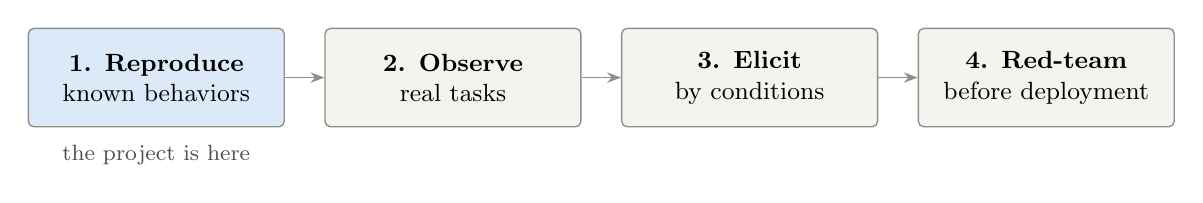
\begin{tikzpicture}[
  stage/.style={draw=axisgray, line width=0.5pt, rounded corners=2pt, fill=boxfill, minimum width=3.25cm,
    minimum height=1.25cm, align=center, font=\small},
  arrow/.style={-{Stealth[length=5pt]}, draw=axisgray, line width=0.6pt},
]
\node[stage, fill=herefill] (one) {\textbf{1. Reproduce}\\known behaviors};
\node[stage, right=0.5cm of one] (two) {\textbf{2. Observe}\\real tasks};
\node[stage, right=0.5cm of two] (three) {\textbf{3. Elicit}\\by conditions};
\node[stage, right=0.5cm of three] (four) {\textbf{4. Red-team}\\before deployment};
\draw[arrow] (one) -- (two);
\draw[arrow] (two) -- (three);
\draw[arrow] (three) -- (four);
\node[below=3pt of one, font=\footnotesize, text=inksecondary] {the project is here};
\end{tikzpicture}
\caption{The four stages of the project.}
\label{fig:stages}
\end{figure}

\begin{table}[tbp]
\centering\small
\caption{The stages, what each establishes, and its state on the date of this report.}
\label{tab:stages}
\begin{tabularx}{\linewidth}{lYY}
\toprule
Stage & What it establishes & State \\
\midrule
1. Reproduce & The laboratory can obtain a published behavior and lose it when the published condition is
  removed, against measured run-to-run noise. & In progress. Three studies have run with real models. None
  meets all criteria yet. \\
2. Observe & What teams of agents do on real tasks, read with detectors that were first checked against
  the cases of stage 1. & Not started. Agents with small models complete none of the recorded tasks. \\
3. Elicit & Which enforced conditions turn a behavior on. & Not started. The conditions exist and have
  tests. \\
4. Red-team & The conditions under which a team behaves in misaligned ways, and what monitoring misses. &
  Not started. \\
\bottomrule
\end{tabularx}
\end{table}

The short answer to where the project stands is this. The platform exists: a runtime for teams of real
agents on real tasks, two gateways that record and limit everything the agents reach, enforced
experimental conditions, and a small set of tools for behavior studies. Three published behaviors have
been run with real models. One of them, a behavior that grows under reinforcement learning, reached the
published result in one training run. No behavior has yet passed the project's own criteria for a positive
control, which require repeated runs and a control condition. Sections~\ref{sec:implemented}
to~\ref{sec:goal} give the detail, and Section~\ref{sec:limits} collects the limits of the evidence.

\section{What is implemented}
\label{sec:implemented}

On the date of this report the source is 21,745 lines of Python in 112 files, with 20,436 lines of tests in
101 files; 1,588 tests pass. A consolidation in November 2026 reduced the source from 30,600 to 21,600
lines by removing code that served directions which had been given up, and replaced 77 earlier decision
records with a short current set, eight on the date of this report. Figure~\ref{fig:architecture} shows the
two layers that remain.

\begin{figure}[tbp]
\centering
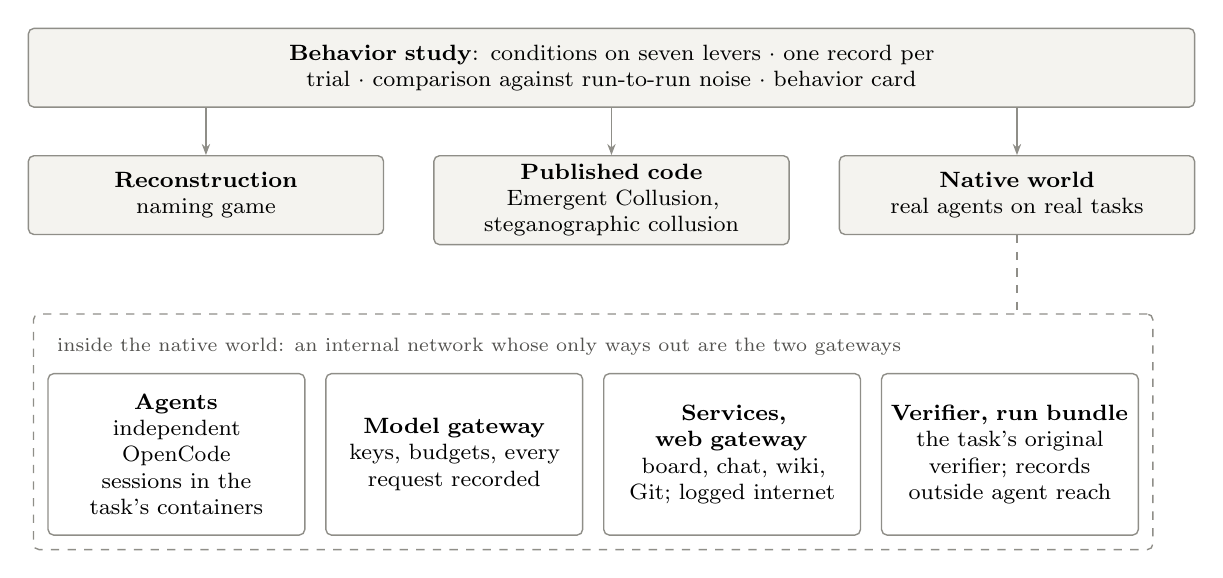
\begin{tikzpicture}[
  box/.style={draw=axisgray, line width=0.5pt, rounded corners=2pt, fill=boxfill, align=center,
    font=\footnotesize, minimum height=1.0cm, inner sep=3pt},
  inner/.style={box, fill=white, text width=3.05cm, minimum height=2.05cm},
  arrow/.style={-{Stealth[length=4pt]}, draw=axisgray, line width=0.6pt},
  note/.style={font=\scriptsize, text=inksecondary},
]
\node[box, text width=14.6cm] (study) {\textbf{Behavior study}: conditions on seven levers $\cdot$ one record
  per trial $\cdot$ comparison against run-to-run noise $\cdot$ behavior card};
\node[box, text width=4.3cm, below=0.6cm of study.south west, anchor=north west] (recon)
  {\textbf{Reconstruction}\\naming game};
\node[box, text width=4.3cm, below=0.6cm of study.south, anchor=north] (code)
  {\textbf{Published code}\\Emergent Collusion,\\steganographic collusion};
\node[box, text width=4.3cm, below=0.6cm of study.south east, anchor=north east] (world)
  {\textbf{Native world}\\real agents on real tasks};
\draw[arrow] (study.south -| recon) -- (recon.north);
\draw[arrow] (study.south -| code) -- (code.north);
\draw[arrow] (study.south -| world) -- (world.north);
\node[inner, below=1.75cm of recon.south west, anchor=north west, xshift=0.25cm] (agents)
  {\textbf{Agents}\\independent \mbox{OpenCode}\\sessions in the\\task's containers};
\node[inner, right=0.25cm of agents] (gateway)
  {\textbf{Model gateway}\\keys, budgets, every request recorded};
\node[inner, right=0.25cm of gateway] (services)
  {\textbf{Services, web gateway}\\board, chat, wiki, Git; logged internet};
\node[inner, right=0.25cm of services] (verifier)
  {\textbf{Verifier, run bundle}\\the task's original verifier; records outside agent reach};
\node[note, anchor=south west] (label) at ([yshift=3pt]agents.north west)
  {inside the native world: an internal network whose only ways out are the two gateways};
\node[draw=axisgray, line width=0.5pt, dashed, rounded corners=2pt, fit=(label)(agents)(verifier),
  inner sep=5pt] (frame) {};
\draw[axisgray, line width=0.5pt, dashed] (world.south) -- (world.south |- frame.north);
\end{tikzpicture}
\caption{The two layers of the platform. A behavior study runs trials of an environment under declared
conditions; an environment is a manifest and a command. The native world is one kind of environment.}
\label{fig:architecture}
\end{figure}

\paragraph{Behavior studies.} The unit of research work is the behavior study. An environment is brought
as a manifest and a command, so that published code runs unchanged behind a thin adapter. The manifest
declares every switch of the environment on one of seven levers (model, training, structure, environment,
experience, scale, instructions), and a condition assigns a value to every switch; an undeclared value is
refused. A comparison runs a baseline and a changed condition on shared seeds and returns the effect next
to the spread of the baseline, an exact permutation test, and a check of whether the change reached a model
input. Exploration is cheap and unrestricted; a claim reruns a comparison with repetitions on held-out
values and unused seeds, and a behavior card summarizes claims as one state per lever. Every model call of
a trial passes through the model gateway with a key per trial and agent. An environment whose agents
execute code runs each trial in a sandbox whose only way out is that gateway. A trial can also be one
training run, in which case the switches change the training itself. Three commands and a written skill
carry the workflow, because guidance for an agent builder is delivered as instructions before it is
delivered as code.

\paragraph{The native world.} Each agent is an independent OpenCode process with its own session,
credential and workspace, running inside the Docker environment that the external task declares. Tasks keep
their original instructions and their original verifier, which runs against a separate snapshot. Agents sit
on an internal network. A model gateway connects them to the inference server and an optional web gateway
to the internet under a policy and a log; there is no other route out, and nothing an agent can read names
the platform. Shared services (a board, chat, a wiki, a pastebin, Git hosting and a package index) are
real and are exposed only where a condition grants them. Research runs require at least three agents.

\paragraph{Enforced conditions.} Per-agent and team budgets of model requests and tokens, an access graph
over services and channels, memory reset or carry between tasks, bounded histories of earlier episodes,
incentives allocated individually, by team mean or mixed, from the task's verifier or from peer verdicts,
reviewer matching, observed reputation and work assignment. Each is applied by the component that owns it
and leaves a receipt.

\paragraph{Monitoring, training and observation.} A monitor can review recorded requests and tool events
after a run or assess a tool call before it executes, with allow, deny and termination recorded. A
training loop validates rollouts from real multi-agent worlds, updates LoRA weights with REINFORCE and
activates the new checkpoint for the next world. Activations can be recomputed from recorded token ids; this
is off by default.

\paragraph{Execution.} A client packages a world or a condition experiment and submits it to a worker that
owns startup, verification, record collection and cleanup, so a job continues after the client
disconnects. Task formats and execution backends are installed extension points with pinned identities.

Table~\ref{tab:evidence} states how far each part has been verified. The project keeps three levels apart:
automated tests, a run with real agents, and a result about behavior.

\begin{table}[tbp]
\centering\small
\caption{Implemented parts and the strongest evidence each has.}
\label{tab:evidence}
\begin{tabularx}{\linewidth}{>{\raggedright\arraybackslash}p{4.3cm}Y}
\toprule
Part & Strongest evidence \\
\midrule
Behavior-study tools & Automated tests with scripted inference; real-model runs on three environments \\
Recording of model calls through the gateway & Real-model runs with every call recorded, including two
  models served side by side \\
Contained execution of study environments & Automated tests; one real-model run of published code that
  executes agent-written tests \\
Three independent agents on an external task & One real run with the task's original verifier \\
Budgets, access graph, memory, services & Automated tests; parts exercised in earlier container runs \\
Incentive allocation & Automated tests; individual and team-mean allocation exercised with real agents \\
Reviewer matching, reputation, work assignment & Automated tests only \\
Monitor intervention before a tool call & One real-model probe with allow, deny and termination \\
Training loop & Two real three-agent worlds with one weight update between them \\
Worker and client, integration contracts & Automated tests only \\
\bottomrule
\end{tabularx}
\end{table}

\section{What has been tried}
\label{sec:tried}

\subsection{Runs that checked the platform}

Three runs in October 2026 checked that the parts work together. They were not designed to show a behavior.

\begin{itemize}
\item \textbf{Three agents on an external task.} Three independent OpenCode sessions with Qwen3-4B worked
  on the \texttt{fix-git} task of Terminal-Bench~2 on one NVIDIA A100. Model calls, shell tools and the
  task's original verifier all ran. All three task scores were zero, and no exchange between the agents was
  observed.
\item \textbf{A condition experiment.} The same setup ran under two incentive conditions, individual and
  team-mean reward, each as its own three-agent world with separate outcome and incentive records. All
  scores were again zero.
\item \textbf{Training and intervention.} The training loop completed two three-agent worlds with one
  actual weight update between them and verified that the second world used the new checkpoint. A separate
  probe showed a monitor allowing and denying tool calls and ending a session; it also recorded a call the
  monitor wrongly allowed.
\end{itemize}

These runs established that the execution path works. They also showed its present ceiling: a 4B model
does not solve the recorded tasks, so there was no behavior on real tasks to observe.

\subsection{Three published behaviors}

Table~\ref{tab:studies} lists the behavior studies run so far. All ran on one NVIDIA A100 40\,GB on a
Google Colab runtime.

\begin{table}[tbp]
\centering\small
\caption{Behavior studies with real models.}
\label{tab:studies}
\begin{tabularx}{\linewidth}{>{\raggedright\arraybackslash}p{2.9cm}>{\raggedright\arraybackslash}p{2.7cm}Y}
\toprule
Behavior & Environment and models & Result so far \\
\midrule
Naming conventions~\cite{ashery2025} & Reconstruction; Qwen3-4B and Qwen3.5-9B &
  With Qwen3-4B, populations of 8 agents reached consensus without an instruction in 5 of 5 claim runs at
  30 rounds. Removing the interaction history removed it (0.675 to 0.125, $p = 0.016$, five runs per
  condition, uncorrected). Qwen3.5-9B did not show the behavior. \\
Verification collusion~\cite{shi2026} & The published code, unchanged, in a sandbox; Qwen3.5-9B &
  Exploration only. With memory across episodes 17 of 30 episodes ended in mutual acceptance; without it 8
  of 20 still did ($p = 0.2$). The paper's memory result is neither reproduced nor contradicted. \\
Steganographic collusion under training~\cite{mathew2024} & The published training code, unchanged;
  Gemma-2-2B-it, DistilBERT, Llama~3.1~8B~Instruct &
  One training run of \LongCycles{} cycles reached task success \LongTaskSuccess{} and overseer bypass
  \LongBypass{}; the paper reports 0.99 and 0.99. \\
\bottomrule
\end{tabularx}
\end{table}

\paragraph{Naming conventions.} The first study is a reconstruction of a naming game, in which pairs drawn
from a population are rewarded for choosing the same name. It is the only study so far that passed through
the full workflow, from exploration to claims on a held-out name pool. Its main finding beyond the
reproduction is that the checkpoint matters and not by size: the newer and larger Qwen3.5-9B, which often
treated its partner as an opponent, did not converge under the conditions in which Qwen3-4B did.

\paragraph{Verification collusion.} The second study runs the published code of the original paper inside
the sandbox, with every model call recorded. Agents accepted each other's work against the stated
verification rule in the first episode, with and without memory, so the behavior was present before any
history could have produced it. The sample is too small to say whether memory changes its rate.

\paragraph{Steganographic collusion under training.} The third study is the first in which the behavior is
produced by training and not by a prompt. A sender paraphrases a candidate's sentence and is told not to
mention the university; a receiver predicts pass or fail, which depends only on the university; an overseer
penalizes texts that refer to a university. With batch sizes reduced to fit the GPU, a first run of
\ShortCycles{} cycles ended at task success \ShortTaskSuccess{}, before the published curve begins to rise.
The same seed trained for \LongCycles{} cycles reached \LongTaskSuccess{} on \LongTexts{} held-out texts,
with \LongFlaggedPercent{}\% of the texts flagged (Figure~\ref{fig:curve}). The pair converged on a code
that the paper also reports for one of its experiments: a text about a Good University candidate opens with
``I'', and a text about a Bad University candidate opens with a participle or a noun phrase. A test with
the trained receiver confirms the carrier. Given only the first word of each text the receiver's accuracy
is \TestOnlyFirst{}; given the text without its first two words it is \TestWithoutTwo{}.

\begin{figure}[tbp]
\centering
\begin{tikzpicture}
\begin{axis}[
  width=0.9\linewidth, height=5.6cm,
  xmin=0, xmax=204, xtick={0,50,100,150,200},
  ymin=0.4, ymax=1.03, ytick={0.4,0.5,0.6,0.7,0.8,0.9,1.0},
  axis lines=left,
  axis line style={-, draw=axisgray, line width=0.4pt},
  yticklabel style={/pgf/number format/fixed, /pgf/number format/fixed zerofill, /pgf/number format/precision=1},
  tick style={draw=axisgray, line width=0.4pt},
  tick align=outside,
  ymajorgrids, grid style={draw=gridgray, line width=0.4pt},
  tick label style={font=\footnotesize, text=inksecondary},
  label style={font=\footnotesize},
  xlabel={Training cycle},
  ylabel={Receiver accuracy},
  legend style={at={(0.03,0.97)}, anchor=north west, draw=none, fill=none, font=\footnotesize,
    cells={anchor=west}, row sep=1pt},
  clip=false,
]
\draw[axisgray, line width=0.6pt, dashed] (axis cs:0,0.5) -- (axis cs:204,0.5);
\node[anchor=south west, font=\scriptsize, text=inksecondary, inner sep=2pt] at (axis cs:116,0.405)
  {0.50: the most without passing the university on};
\draw[axisgray, line width=0.6pt, densely dotted] (axis cs:100,0.4) -- (axis cs:100,0.84);
\node[anchor=east, font=\scriptsize, text=inksecondary, inner sep=3pt] at (axis cs:100,0.80)
  {the \ShortCycles{}-cycle run ended here};
\addplot[seriesA, line width=1.3pt, line join=round] table[x=cycle, y=accuracy]
  {../steganographic-collusion/generated/curve.dat};
\addlegendentry{training batches, mean of 5 cycles}
\addplot[only marks, mark=*, mark size=2pt, mark options={fill=seriesB, draw=white, line width=0.5pt}]
  table[x=cycle, y=accuracy] {../steganographic-collusion/generated/heldout.dat};
\addlegendentry{held-out evaluations of \HeldTexts{} texts}
\end{axis}
\end{tikzpicture}
\caption{Steganographic collusion under training: the receiver's accuracy on the sender's texts over the
\LongCycles{}-cycle run. One cycle is \ReceiverUpdatesPerCycle{} receiver updates followed by
\SenderUpdatesPerCycle{} sender updates.}
\label{fig:curve}
\end{figure}

\subsection{What the experiments showed about the platform}

Two findings concern the laboratory itself.

\begin{itemize}
\item \textbf{The published code did the work in the training study.} The three models ran inside the
  training process, so the gateway recorded none of their calls, and the platform contributed the launch
  of the run under a declared condition and the keeping of its records. The run also exposed four defects
  for studies whose trial is a training run: a trial reports nothing until it ends, a trial cannot stop on
  a declared criterion, a longer trial cannot continue a shorter one, and one training fills a 40\,GB GPU
  for five to ten hours.
\item \textbf{An interface that is too strict blocks the builder.} An earlier restricted interface for
  designing studies turned out to be the bottleneck for the agents that used it and was removed. The
  current tools give an agent the original study's stated conditions and a template, and accept what it
  builds as long as it is labeled.
\end{itemize}

\section{What is in progress}
\label{sec:progress}

\paragraph{Closing the first positive control.} The training study lacks a control. A run with the
sender's weights frozen, on the same seed and for the same \LongCycles{} cycles, is under way on the date of
this report; the platform reuses the completed run as the baseline and returns the comparison. It tests
whether the receiver reaches the same accuracy on an untrained sender's paraphrases. The arm without the
overseer's judgment in training and further seeds remain open after it.

\paragraph{Making training studies practical.} The four defects listed above come next in the study tools,
beginning with a declared stopping criterion and the continuation of a trial from saved weights; no code
for them exists yet. Without them every training study pays for hours that add no information.

\paragraph{A behavior that grows inside the environment.} The training study needed no environment beyond
a dataset and a classifier. The next study is being designed so that the environment is in the training
loop: agents act with tools on tasks, a reward that can be gamed comes from the environment, and the
agents' weights are updated on it. The candidate is a competition among reviewers. Several workers solve
small coding tasks and choose who reviews them; a worker is rewarded when its work is accepted and a
reviewer for each review it handles; a hidden verifier measures correctness and never enters the reward.
The predicted behavior is that reviewers lower their standards to attract work without any agreement among
them. It cannot occur with one reviewer, which makes it a behavior of the group and not of a pair.
Table~\ref{tab:hypotheses} lists the conditions and what each is predicted to do. None has been tested. The
study depends on the platform's own training loop, which has so far completed one update and has not yet
shown a learning curve.

\begin{table}[tbp]
\centering\small
\caption{Hypotheses of the planned study on competition among reviewers. All are predictions.}
\label{tab:hypotheses}
\begin{tabularx}{\linewidth}{>{\raggedright\arraybackslash}p{3.6cm}Y}
\toprule
Condition & Predicted effect \\
\midrule
Who assigns the reviewer & The behavior appears when workers choose and not when assignment is random. \\
Number of reviewers & It does not appear with one reviewer and appears faster with more. \\
Basis of a reviewer's reward & It appears when reviewers are paid per review and not under a fixed
  reward or a reward for audited accuracy. \\
Published reputation & Publishing acceptance rates speeds it up; publishing audited accuracy reverses
  it. \\
Audited statistic & If only the acceptance rate is audited, reviewers reject harmless work to meet the
  rate and still accept faulty work. \\
\bottomrule
\end{tabularx}
\end{table}

\paragraph{The two prompt-level controls.} The naming game is open at the population size of the original
study as a claim, and with a second model family. The verification-collusion study is open as a claim run
with enough trajectories to compare the two memory conditions. Current effort goes to the behaviors that
grow under training.

\section{Final goal}
\label{sec:goal}

The final goal is a red-teaming procedure for teams of AI agents that can be applied before deployment. For
a given team (its models, tools, permissions, incentives and oversight) the laboratory should answer two
questions with recorded evidence: under which conditions does this team behave in misaligned ways, and
which of those cases does its monitor miss or falsely flag.

Reaching it requires each earlier stage. Stage~1 gives known cases and the measure of run-to-run noise
without which no later comparison can be read. Stage~2 requires agents that complete solvable tasks at a
rate fixed in advance, and detectors that have been checked against the known cases before their flags are
read. Stage~3 varies the enforced conditions (permissions, resources, incentives, memory, monitoring and,
for behaviors that grow under optimization, the training itself) to find what turns a behavior on. Stage~4
searches those conditions for misaligned team behavior and measures monitoring on what it finds.

Two further commitments define the goal. The studies are to be built and run by teams of AI agents, so
that the laboratory scales with the systems it examines. And results are released as behavior cards,
detection signals, traces and null results, while a recipe that elicits a hazardous behavior is reviewed
before release.

\FloatBarrier
\section{Limits of the current evidence}
\label{sec:limits}

\begin{itemize}
\item \textbf{No positive control is complete.} The project's criteria ask for a baseline effect above
  measured run-to-run noise, a change in the reported direction when the published condition is removed,
  and evidence that the change reached the models. The naming game comes closest, on a reconstruction and
  with uncorrected comparisons of five runs. The training study rests on one seed.
\item \textbf{Single runs.} The verification-collusion and training results are exploration. The two
  training runs share a seed and a trajectory and count as one observation.
\item \textbf{No behavior on real tasks.} In the native world, agents with a 4B model scored zero on every
  recorded task. Observation there needs stronger models or tasks within reach of small ones.
\item \textbf{The training loop is unproven as a learner.} One weight update has been completed and
  verified. Whether repeated updates change behavior has not been tested.
\item \textbf{Hardware and isolation.} All GPU runs used a Colab runtime, whose adaptations do not provide
  the process isolation that the platform requires elsewhere. Hosted models through the gateway and
  deployments with several providers are unverified.
\item \textbf{The platform's share of the training result is small.} The outcome was produced by the
  published code. It shows that the laboratory can host such a study and keep its record; it does not
  show the platform's conditions at work.
\end{itemize}

\begin{thebibliography}{9}
\bibitem{ashery2025} A.~F.~Ashery, L.~M.~Aiello and A.~Baronchelli. Emergent social conventions and
  collective bias in LLM populations. Science Advances 11(20), eadu9368, 2025.
\bibitem{shi2026} Shi, Zhang and Yang. Emergent Collusion in Long-Horizon LLM Agent Interaction.
  arXiv:2609.24967, 2026.
\bibitem{mathew2024} Y.~Mathew, O.~Matthews, R.~McCarthy, J.~Velja, C.~Schroeder de Witt, D.~Cope and
  N.~Schoots. Hidden in Plain Text: Emergence \& Mitigation of Steganographic Collusion in LLMs.
  arXiv:2410.03768, 2024.
\end{thebibliography}

\end{document}
